\documentclass[12pt]{article}
\usepackage{mathtools, amsmath, amsfonts, amssymb, siunitx,array}
\usepackage{hyperref, graphicx, wrapfig, geometry}
\usepackage[makeroom]{cancel}
\usepackage{placeins}
\usepackage{float}


\newgeometry{margin=2cm}

\title{Microprocessor Systems - Project Lab Report}
\author{Auguste Lalande, Felix Dube, Juan Morency Trudel}
\date{\today}

\begin{document}
\maketitle
\clearpage

\tableofcontents
\clearpage

\section{Abstract}

\section{Problem Statement}

\section{Theory and Hypothesis}
\subsection{Bluetooth Low Energy}
Bluetooth Low Energy allows the wireless communication between different devices. The Generic Attribute Profile (GATT) is the protocol used to exchange data over BLE connection. First of all, GATT defines the different roles that the connected devices can adopt. On one hand, a device can be Client. In this role, the device sends request to a server and receives responses from it. On the other hand, a device can be a Server. In this role, the device receives and sends responses to the clients. It is also responsible for storing and making the data available to the client.

Moreover, GATT uses the Attribute Protocol (ATT) as its transport protocol. The ATT defines how the data is organised. In the GATT server data are separated in different section called services. Each services holds one to many characteristics, and these characteristics are what contains the user data. Figure \ref{fig:gatt} illustrate the data structure introduced by GATT.

\begin{figure}[!htb]
 \centering
 \includegraphics[scale=0.65]{images/GATT.png}
 \caption{GATT Server Overview}
 \label{fig:gatt}
\end{figure}

Each characteristics can have different properties. A characteristic can have Read property, which means that a client can read the data that it contains. It can also have Write property where the user can modify the data that the characteristic holds. Moreover, a characteristic can have the notify property, which allow the server to do a notification operation on it.

\subsection{Android}
An Android phone is a good device to use as a user interface since the view can be change for each application. It also allow to communicate with other devices using many different wireless communication protocol, including BLE which was used for this lab. Additionally, Android application can be easily build using Android Studio.

\subsection{SPI Communication}
The serial peripheral interface (SPI) protocol is a four wire, full duplex, serial interface specification ideal for short range communication between embedded devices.As seen in figure \ref{fig:spi}, the implementation uses two data lines, one clock line, and one slave select line. The data lines are divided into the master in slave out (MISO) which is driven by the slave and the master out slave in (MOSI) which is driven by the master. All communication is synced to the master's clock which is set on the clock line (SCLK). Finally the slave select line (SSL) is used by the master to indicate which slave it is communicating with. In the case where there is only one slave the line can be kept permanently high. 

\begin{figure}[!htb]
 \centering
 \includegraphics[scale=0.65]{images/spi.png}
 \caption{SPI Communication Overview}
 \label{fig:spi}
\end{figure}

\section{Implementation}
\subsection{Bluetooth Low Energy}
For this lab, the GATT server was managed by the Nucleo board using the X-NUCLEO-IDB04A1 Bluetooth shield and only one client, the Android phone, was interacting with the server. An overview of the GATT server can be seen in figure \ref{fig:gattimp}.

\begin{figure}[!htb]
 \centering
 \includegraphics[scale=0.65]{images/GATTimplementation.png}
 \caption{GATT Server Implementation}
 \label{fig:gattimp}
\end{figure}

The accelerometer service allowed the phone to read the roll and pitch values, which were updated by the Nucleo board. Similarly, the phone would receive information about the temperature of the CPU. The GATT server also holds an LED service, which contains characteristic for which the value would be updated by the phone. Lastly the Nucleo board can notify the phone using the double tap service, which contains only one characteristic.

\subsection{Android}
The user interface have been implemented using Android Studio, and tested on a Samsung Galaxy S6 phone. Using the phone the user can control different behavior of the discovery board, and receive data from it. An overview of the application can be seen in figure \ref{fig:android}.

\begin{figure}[!htb]
 \centering
 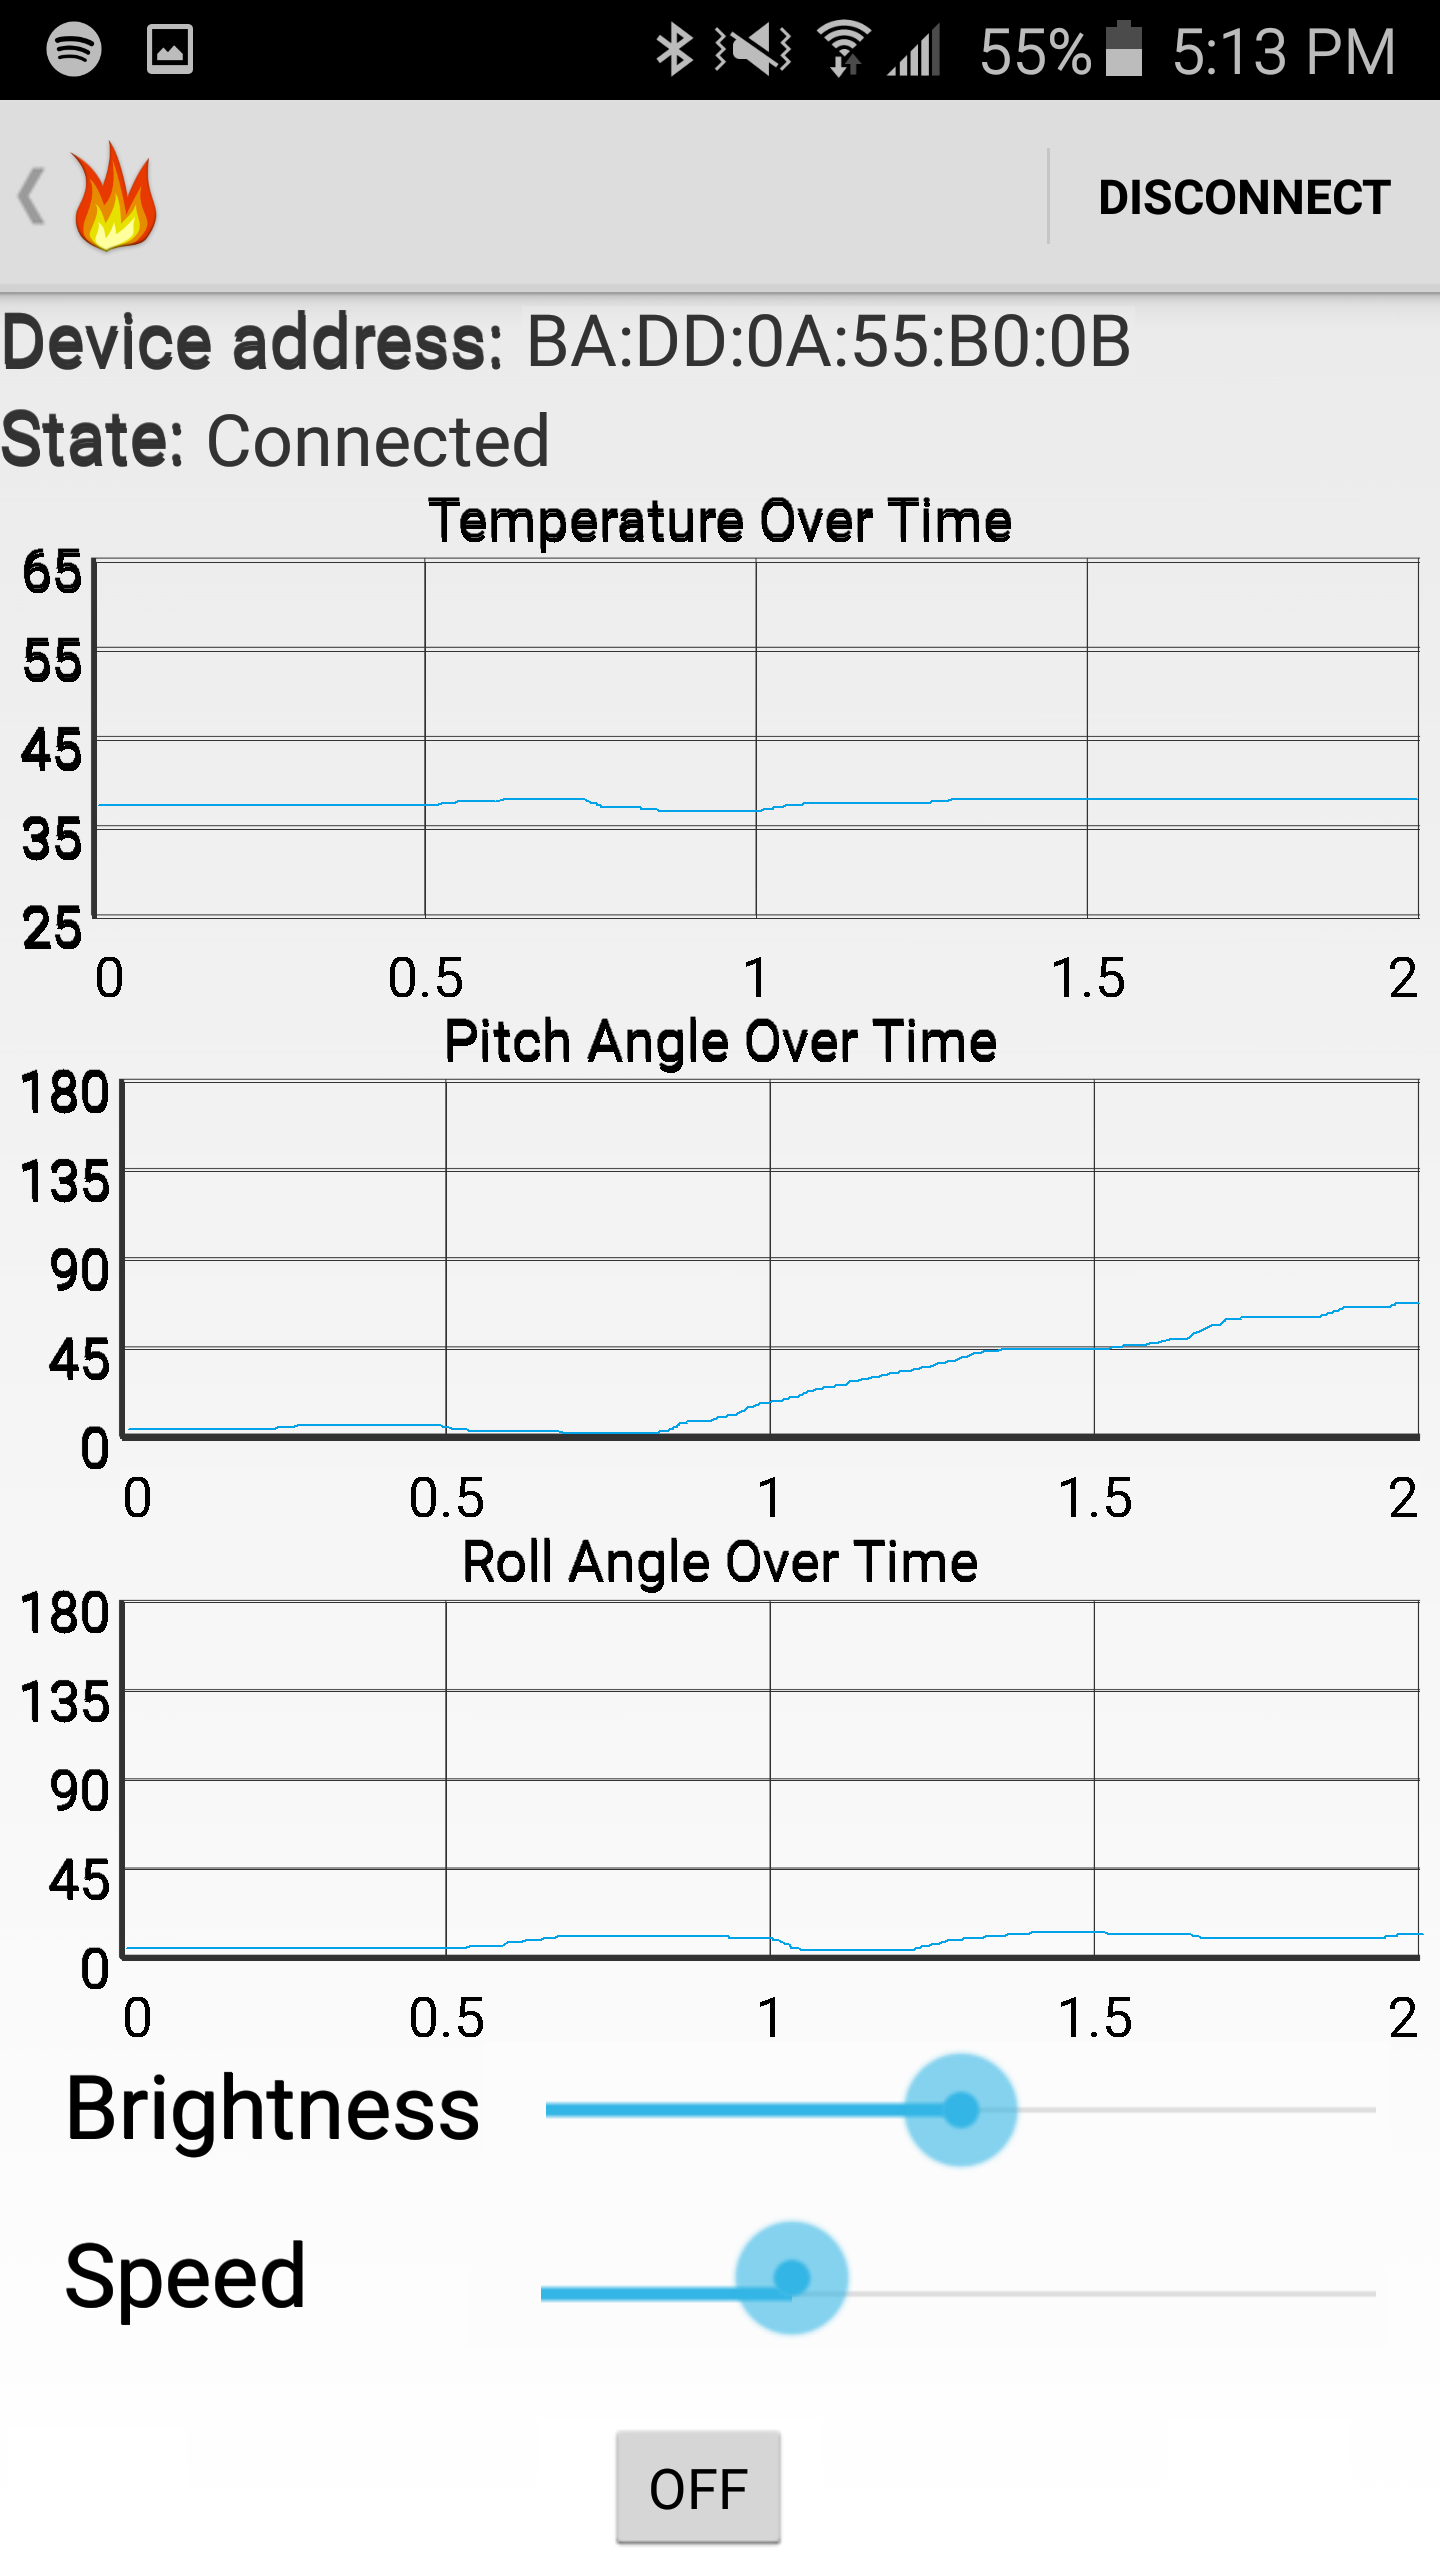
\includegraphics[scale=0.15]{images/android.png}
 \caption{Android Application Main View}
 \label{fig:android}
\end{figure}

First of all, the temperature, roll, and pitch data are presented to the user using graph from the Graph View library. For each of the values, a tread have been setup to read the Bluetooth characteristic and update the data points that are displayed on the graph every 20 milliseconds. The main thread would then update the view with the new data points.

Secondly, the view contains two sliders, which control the speed and brightness of the LEDs on the Discovery board. A listener has been instantiated for each of the sliders. When the user moves a slider the listener call a function that write the new value to the specific characteristic. The view also contains a button. When it is pressed the function that writes to the on/off characteristic is being called. This allows the user to change the state of the LEDs.

Lastly, when the double tap characteristic is being notified an Android notification is being displayed on the screen. If the phone is sleeping, the screen wakes up to display the notification.

\subsection{SPI Communication}
SPI communication was used to transfer data between the discovery board and the Nucleo board. It was important for the two boards to be able to communicate because only the Nucleo board was equipped with Bluetooth capabilities while the discovery board was used to acquire data.

Although HAL drivers were available which already implemented SPI communication, these were found to be difficult to use. Therefore the communication was implemented without the use of said drivers. A simple protocol was implemented whereby the Nucleo board would wait for a START\_BYTE indicating the beginning of communication, after which all data was transferred between the boards one byte at a time. In the case where the data to be communicated was a float, the discovery board would first convert the IEEE 754 number into a byte array which could then be transferred and converted back to a float by the Nucleo board.

\section{Testing and Observations}

\section{Timeline and Work Breakdown Between Team Members}

\section{Conclusion}

\newpage
\section{Bibliography}
\bibliographystyle{unsrt}
%\bibliography{}

\newpage
\section{Appendix}
\begin{figure}[!htb]
 \centering
 \includegraphics[scale=0.6]{images/softwareArchitecture.png}
 \caption{High Level View of the Software Architecture}
 \label{fig:softArch}
\end{figure}

\end{document}
